\documentclass[../Main/main.tex]{subfiles}
\begin{document}
	\graphicspath{{../Equivalence between MPFA-L and FEM/figs/}}
	\chapter{Equivalence between MPFA-L and FEM}
		This chapter is adapted from (Cao Wolmuth \cite{https://doi.org/10.1002/num.20525},2009).
		We prove the equivalence for the elliptic model problem \eqref{eq:elliptic model} on homogeneous media discretized by a parallelogram grid.
	\begin{equation}\label{eq:elliptic model 2}
		\begin{aligned}[c]
			- \nabla \cdot \pmb{K} \nabla u(x) &= F(x) \\
			u(x) &= 0 \\
			\pmb{K}\nabla u(x) &= g_N
		\end{aligned}
		\ \ \
		\begin{aligned}[c]
			x &\in \Omega  \\
			x &\in \Gamma_D \\
			x &\in \Gamma_N
		\end{aligned}
	\end{equation}	
	We will need to modify the MPFA-L method on the Neumann boundaries, this is to be expected as finite element methods have degrees of freedom on the boundaries as opposed to finite volume methods. We will also see how we could enforce Dirichlet boundary conditions in a way that is equivalent to the finite element method.

	\section*{Modified MPFA-L method}

	Consider the control volume $y_1 y_6 y_4 y_3$. 
	\begin{figure}[H]
		\centering
		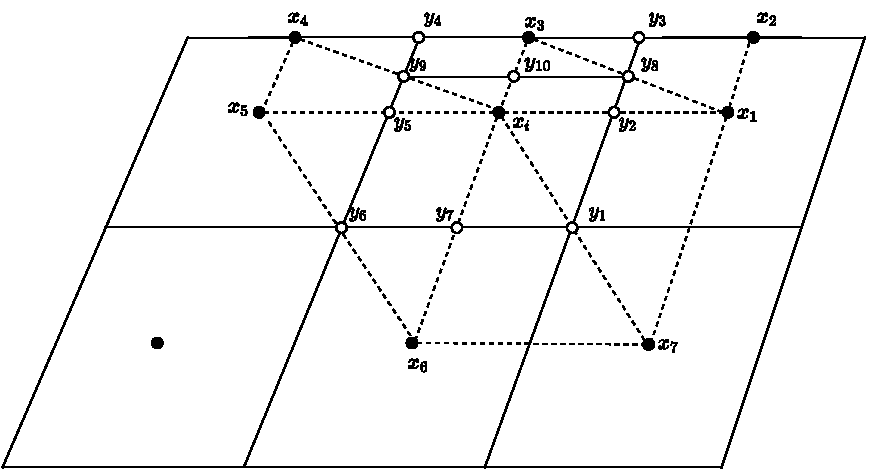
\includegraphics{modified_L_scheme.pdf}
		\caption{Control volumes in solid lines and interaction regions in dashed lines at the boundary.}
	\end{figure}
	For the \textbf{Neumann} boundary conditions, we split the cell into two, $y_1 y_6 y_5 y_2$ as $K_1$ and $y_8 y_9 y_4 y_3$ as  $K_2$. For the fluxes on $K_1$ we have six interaction triangles and a normal seven point stencil. For the $K_2$ we compute the flux trough $\overline{y_3 y_8}$ using $\triangle x_1 x_3 x_2$, the flux trough $\overline{y_8 y_{10}}$ using $\triangle x_1 x_i x_3$, for $\overline{y_{10}y_9}$ and $\overline{y_9 y_4}$ the L triangle  $\triangle x_i x_4 x_3$ is used. Finally the Neumann boundary condition is used at the the edge $\overline{y_4 x_3}$ and $\overline{x_3 y_3}$. We are not able to eliminate the unknown value at $x_3$ and it remains a degree of freedom, which makes sense if we want equivalence with finite element method.
	\par
	In the case of \textbf{Dirichlet} boundary conditions, we compute the fluxes into $y_1 y_6 y_4 y_3$ using seven L-triangles. The flux over the edge $\overline{y_3 y_1}$ are computed as the sum of the flux over $\overline{y_3 y_8}$, $\overline{y_8 y_2}$ and $\overline{y_2 y_1}$ using the L-triangles $\triangle x_1 x_3 x_2$, $\triangle x_1 x_i x_3$ and $\triangle x_1 x_7 x_i$ respectively. Similarly for the edge $\overline{y_6 y_4}$. For $\overline{y_1 y_6}$ we only use the two big L-triangles at the bottom. 
	\par 
	The flux over $\overline{y_4 y_3}$, at the boundary, we compute by balancing it by the other fluxes into the small control volume $K_2$. Let $	f_{\overline{y_i y_j}}:= \int_{\overline{y_i y_j}}  \pmb{K}\nabla u \cdot \pmb{\hat{n}}\ dx $
	\begin{equation}\label{eq:K2}
		f_{\overline{y_4 y_3}} = f_{\overline{y_3 y_8}} + f_{\overline{y_8 y_{10}}}+f_{\overline{y_{10}y_9}}+f_{\overline{y_9 y_4}}
	\end{equation}
	The fluxes on the right hand side of \eqref{eq:K2} are computed as for the Neumann case.
	\section*{Equivalence of stiffness matrix}
	In this section we show that the stiffness matrix arising from the MPFA-L method is equivalent to that of the finite element method we defined in chapter 2. With test space
	\begin{equation}
		V_h = \left \{ v \in C(\Omega): v|_K\in \mathcal{P}_1 \ \ v|_{\Gamma_D}=0 \right \}
	\end{equation}
	The triangulation $\tau_h$ is exactly the L-triangles chosen in the L-method, with the nodes being the cell centres and boundary nodes. We index our nodes with 
	\begin{equation}
		\mathcal{N} = \mathcal{N}^* \bigcup \mathcal{N}^D\bigcup \mathcal{N}^N
	\end{equation}
	Where $\mathcal{N}^*$ are the nodes corresponding to cell centres, we divide further into cells at the boundary and interior cells:
	\begin{equation}
		\mathcal{N}^* = \mathcal{N}^i \bigcup \mathcal{N}^b
	\end{equation}
	\begin{figure}[H]
		\centering
		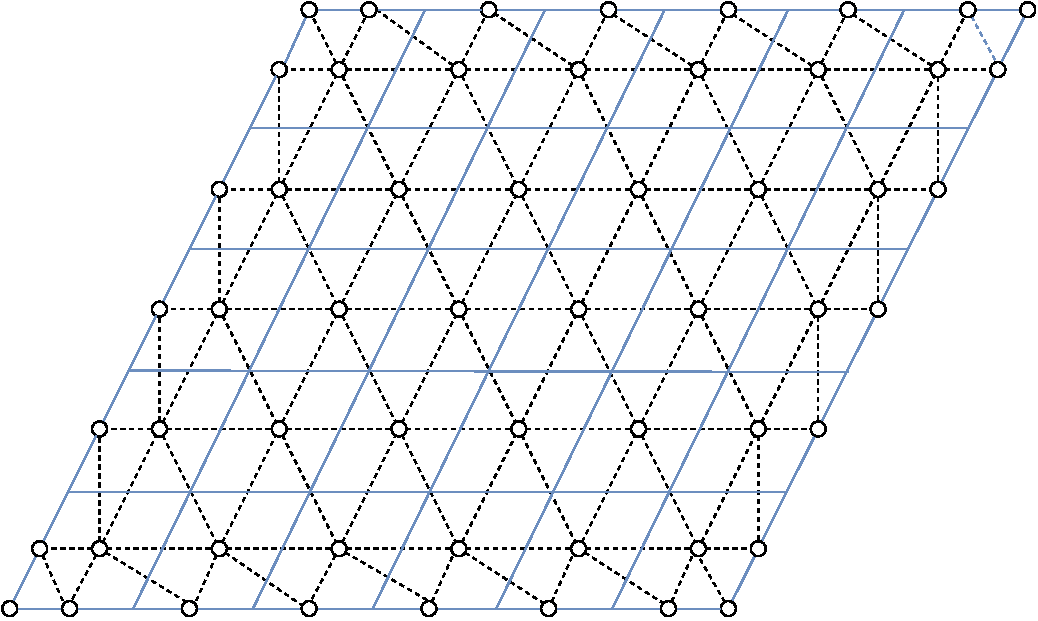
\includegraphics[width=0.8\textwidth]{grid.pdf}
		\caption{The solid lines are control volumes, the dashed lines are the elements/L-triangles.}
	\end{figure}
	Our bi-linear form now becomes, as before
	\begin{equation}\label{eq:bi linear}
		a_h(u,v) = \int_{\Omega}(\nabla u)^T \pmb{K}\nabla v \ dx \ \ u,v \in V_h
	\end{equation}
	And the right hand side is modified with mass lumping 
	\begin{equation}
		b_h(v) = \int_{\Omega} f \hat{I}_h v \ dx + \int_{\Omega }g_N \hat{I}_h v \ dx
	\end{equation}
	Where $\hat{I}_h$ as before restricts $v$ to it's cellcentre value and zero outside it's cell.
	\par
	As our goal is to obtain convergence rate estimates for the MPFA-L method, we assume that we are given $\pmb{K}(x)$ that are piecewise constant in each control volume. But if this is the case, we are no longer able to evaluate the bilinear form exactly, to mediate this we construct a new permeability that is piecewise constant on each triangle and denote it by $\pmb{\hat{K}}(x)$. We will later see that it can be chosen such that we get equivalence with the MPFA-L discretization with the original permeability $\pmb{K}(x)$. To simplify we will often make use of the fact that the permeability only varies as a scalar field and write it as $K(x)$
	\begin{figure}[H]\label{fig:control volume}
		\centering
		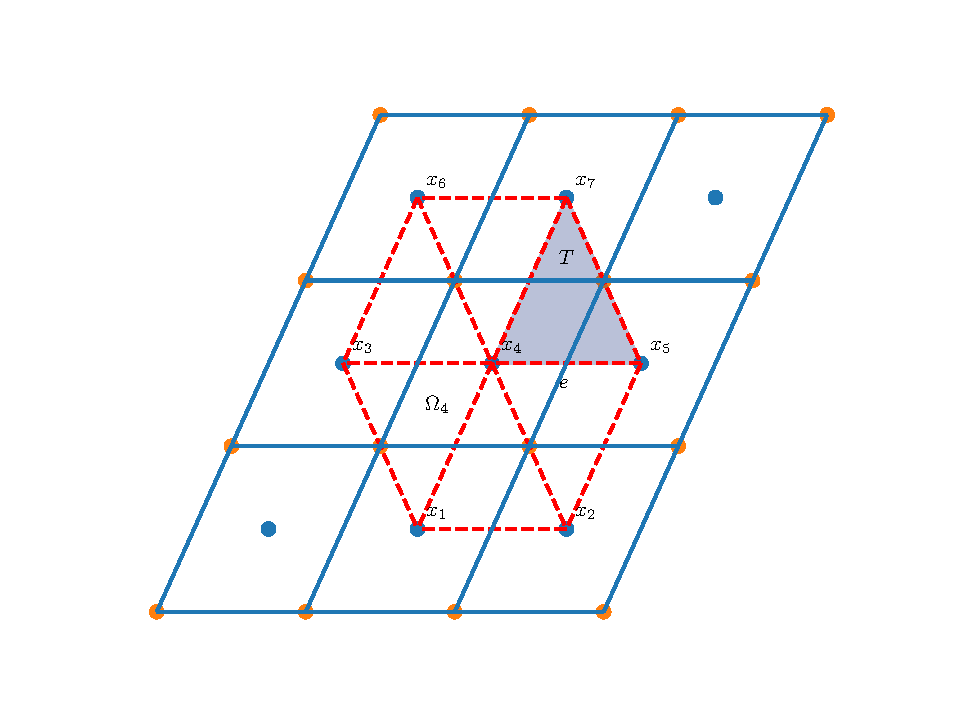
\includegraphics[width=1\textwidth]{Control volume.pdf}
		\caption{The support of $\phi_4$}
	\end{figure}
	\begin{figure}[H]\label{fig:two triangles}
		\centering
		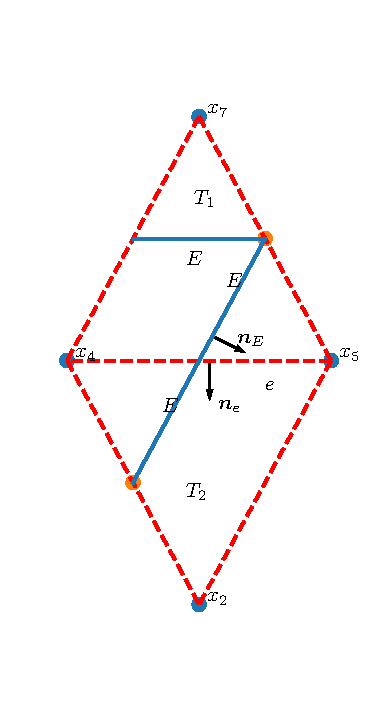
\includegraphics{two triangles.pdf}
		\caption{Notation in the proof}
	\end{figure}
	\begin{lemma}\label{lemma:caowolmuth}
	Let $\phi_i$ be the standard nodal basis function of $V_h$, then:
		\begin{equation}
			a_h(u_h,\phi_i) = \sum_{E \in \partial \Omega_i} -\pmb{\hat{K}}\nabla u_h \cdot \pmb{n}_E |E| \forall i \in \mathcal{N}^*
		\end{equation}
		Where $u_h$ is the solution to 
		\begin{equation}\label{eq:assumption}
		a(u_h,\phi_i) = \int_{\Omega}(\nabla u_h)^T \pmb{\hat{K}}\nabla \phi_i \ dx = \int_{\Omega} f \hat{I}_h \phi_i \ dx = \left\langle f,\hat{I}_h \phi_i \right \rangle_0
		\end{equation}
	\end{lemma}
	\begin{proof}
			\item Let $\Omega_i$ be an interior control volume and $\phi_i$ be the corresponding basis function evaluating to one at the centre of $\Omega_i$, ie. $i \in \mathcal{N}^i$. $T \in tau_h \bigcap \text{supp}(\phi_i)$ is an element of the triangulation. $S=T\bigcap \Omega_i$ and $E \subset S\bigcap \partial \Omega_i$ are the half edges of $\Omega_i$. $e$ are the interior edges of $\tau_h$ inside the support of $\phi_i$, see fig \ref{fig:two triangles} and \ref{fig:control volume}. Since $u_h$ and $\phi$ is piecewise linear and $\pmb{\hat{K}}$ is constant on each triangle $T$ we have:
			\begin{equation}\label{eq:big computation}
				\begin{aligned}
					a_h(u_h,\phi_i) &= \int_{\text{supp}(\phi_i)} (\nabla u_h)^T \pmb{\hat{K}}\nabla \phi_i \ dx = \sum_{T\in \text{supp}(\phi_i)} \int_T (\nabla u_h)^T \pmb{\hat{K}}\nabla \phi_i \ dx \\
					&= \sum_{T\in \text{supp}(\phi_i)} \left ( \int_{\partial T} (\pmb{\hat{K}}\nabla u_h)^T \pmb{n}\phi_i \ ds-\int_T \nabla \cdot \pmb{\hat{K}} \nabla u_h \phi_i \ dx \right ) \\
					&=\sum_{T\in \text{supp}(\phi_i)}\int_{\partial T} (\pmb{\hat{K}}\nabla u_h)^T \pmb{n}\phi_i \ ds \\
					&= \sum_{e\in \text{supp}(\phi_i)} \int_e ((\pmb{\hat{K}}\nabla u_h)^T \pmb{n}_e|_{T_{j}} - (\pmb{\hat{K}}\nabla u_h)^T \pmb{n}_e|_{T_{j+1}})\phi_i \ ds\\
					&= \sum_{e\in \text{supp}(\phi_i)}
					((\pmb{\hat{K}}\nabla u_h)^T \pmb{n}_e|_{T_{j}} - (\pmb{\hat{K}}\nabla u_h)^T \pmb{n}_e|_{T_{j+1}}) \frac{|e|}{2}\\
					&=\sum_{S\in \text{supp}(\phi)}\int_{\partial S}  (\pmb{\hat{K}}\nabla u_h)^T \pmb{n} \ ds - \sum_{E\in \partial \Omega_i}\int_E (\pmb{\hat{K}}\nabla u_h)^T \pmb{n}_E \ ds\\
					&= \sum_{S\in \text{supp}(\phi)}\int_{ S} \nabla \cdot \pmb{\hat{K}}\nabla u_h \ ds - \sum_{E\in \partial \Omega_i}\int_E (\pmb{\hat{K}}\nabla u_h)^T \pmb{n}_E \ ds\\
					&=- \sum_{E\in \partial \Omega_i} (\pmb{\hat{K}}\nabla u_h)^T \pmb{n}_E |E| 
				\end{aligned}
			\end{equation}
	\end{proof}
\end{document}